% Drawing 146/04-8 -- folder 146, batch 04, archive page 66 (PDF page 67).
% Transcription: Un quadrilatère de sommets $0, 1, \infty$ (et un quatrième), coupé par une diagonale, deux régions hachurées ; une ellipse traversée par le segment $1 \;\text{---}\; 0 \;\text{---}\; \infty$, l'arc supérieur marqué $r$, avec l'inscription $\sigma_0 r = \sigma_1 r$.
% Kind: quadrilateral / map on the sphere. Method 2 (schematic redraw from the facsimile). Status: ok.
% Notes: On the upside-down half of the page; redrawn upright. Quadrilateral 0, 1, infinity and a fourth vertex, cut by a diagonal, a second triangle on the right, two hatched (zigzag) regions; the stroke going up from 0 is drawn. Ellipse crossed by the segment 1 -- 0 -- infinity (the 0 -- infinity part thick), upper arc r, inscription sigma0 r = sigma1 r. A loose mark at the left of the ellipse is left out. Not encoded: the figure illustrates the relation sigma0 r = sigma1 r on one edge, not a whole map.
% Coordinates: 1 unit = 1 mm = 1/100 of the crop width (bbox in page fractions: [0.72, 0.62, 0.9, 0.81]).
% Redrawn by Claude (claude-opus-5-5), issue #73 pilot, 2026-11-07; not checked by a human; not compiled (no TeX in the session).
% Rights: reproduces part of the work -- behind RENDER_TRANSCRIPTS, never published by itself.
\documentclass[tikz,border=3pt]{standalone}
\usepackage{amsmath,amssymb}
\usetikzlibrary{patterns,arrows.meta}
\tikzset{pencil/.style={black!45}, struck/.style={black!35}, mark/.style={circle,draw,inner sep=1.3pt}, pt/.style={circle,fill,inner sep=0.9pt}, opt/.style={circle,draw,fill=white,inner sep=1.1pt}}
\begin{document}
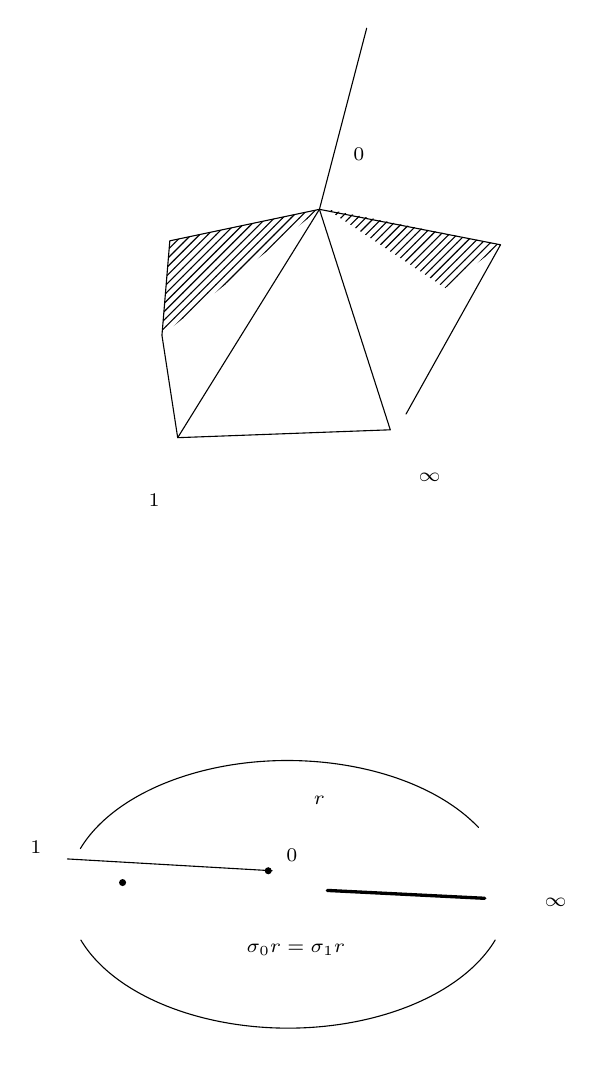
\begin{tikzpicture}[x=1mm,y=1mm,line cap=round,line join=round,font=\scriptsize]
\draw (40,-27) -- (39,-39) -- (41,-52) -- (68,-51) -- (59,-23) -- cycle;
\draw (41,-52) -- (59,-23);
\draw (59,-23) -- (82,-27.5) -- (70,-49);
\draw (59,-23) -- (65,0);
\fill[pattern=north east lines] (40,-27) -- (59,-23) -- (39,-39) -- cycle;
\fill[pattern=north east lines] (60,-23) -- (82,-27.5) -- (75,-33) -- cycle;
\node[inner sep=1pt] at (64,-16) {\scriptsize $0$};
\node[inner sep=1pt] at (73,-57) {\scriptsize $\infty$};
\node[inner sep=1pt] at (38,-60) {\scriptsize $1$};
\draw (79.2,-101.5) arc[start angle=30, end angle=160, x radius=28, y radius=17];
\draw (28.7,-115.8) arc[start angle=200, end angle=340, x radius=28, y radius=17];
\draw (27,-105.5) -- (53,-107);
\draw[very thick] (60,-109.5) -- (80,-110.5);
\node[pt] at (52.5,-107) {};
\node[pt] at (34,-108.5) {};
\node[inner sep=1pt] at (55.5,-105) {\scriptsize $0$};
\node[inner sep=1pt] at (23,-104) {\scriptsize $1$};
\node[inner sep=1pt] at (89,-111) {\scriptsize $\infty$};
\node[inner sep=1pt] at (59,-98) {\scriptsize $r$};
\node[inner sep=1pt] at (56,-117) {\scriptsize $\sigma_0 r=\sigma_1 r$};
\end{tikzpicture}
\end{document}
